\documentclass{standalone}
%
\usepackage{tikz}
\usetikzlibrary{backgrounds}
\usepackage{tkz-euclide}
\usetkzobj{all}
%
\usepackage{amsmath}
%
\usepackage{xcolor}
%
\definecolor{space}{HTML}{0A2543}
\definecolor{earth}{HTML}{0089FA}
\definecolor{mars}{HTML}{DC7B4E}
\definecolor{dida}{HTML}{FFDE00}
\definecolor{title}{HTML}{FBA706}
\definecolor{moon}{HTML}{AFAFAF}
%
\usepackage{fontspec}
\setmainfont{Montserrat}
%
\title{Square roots without words}
\begin{document}
	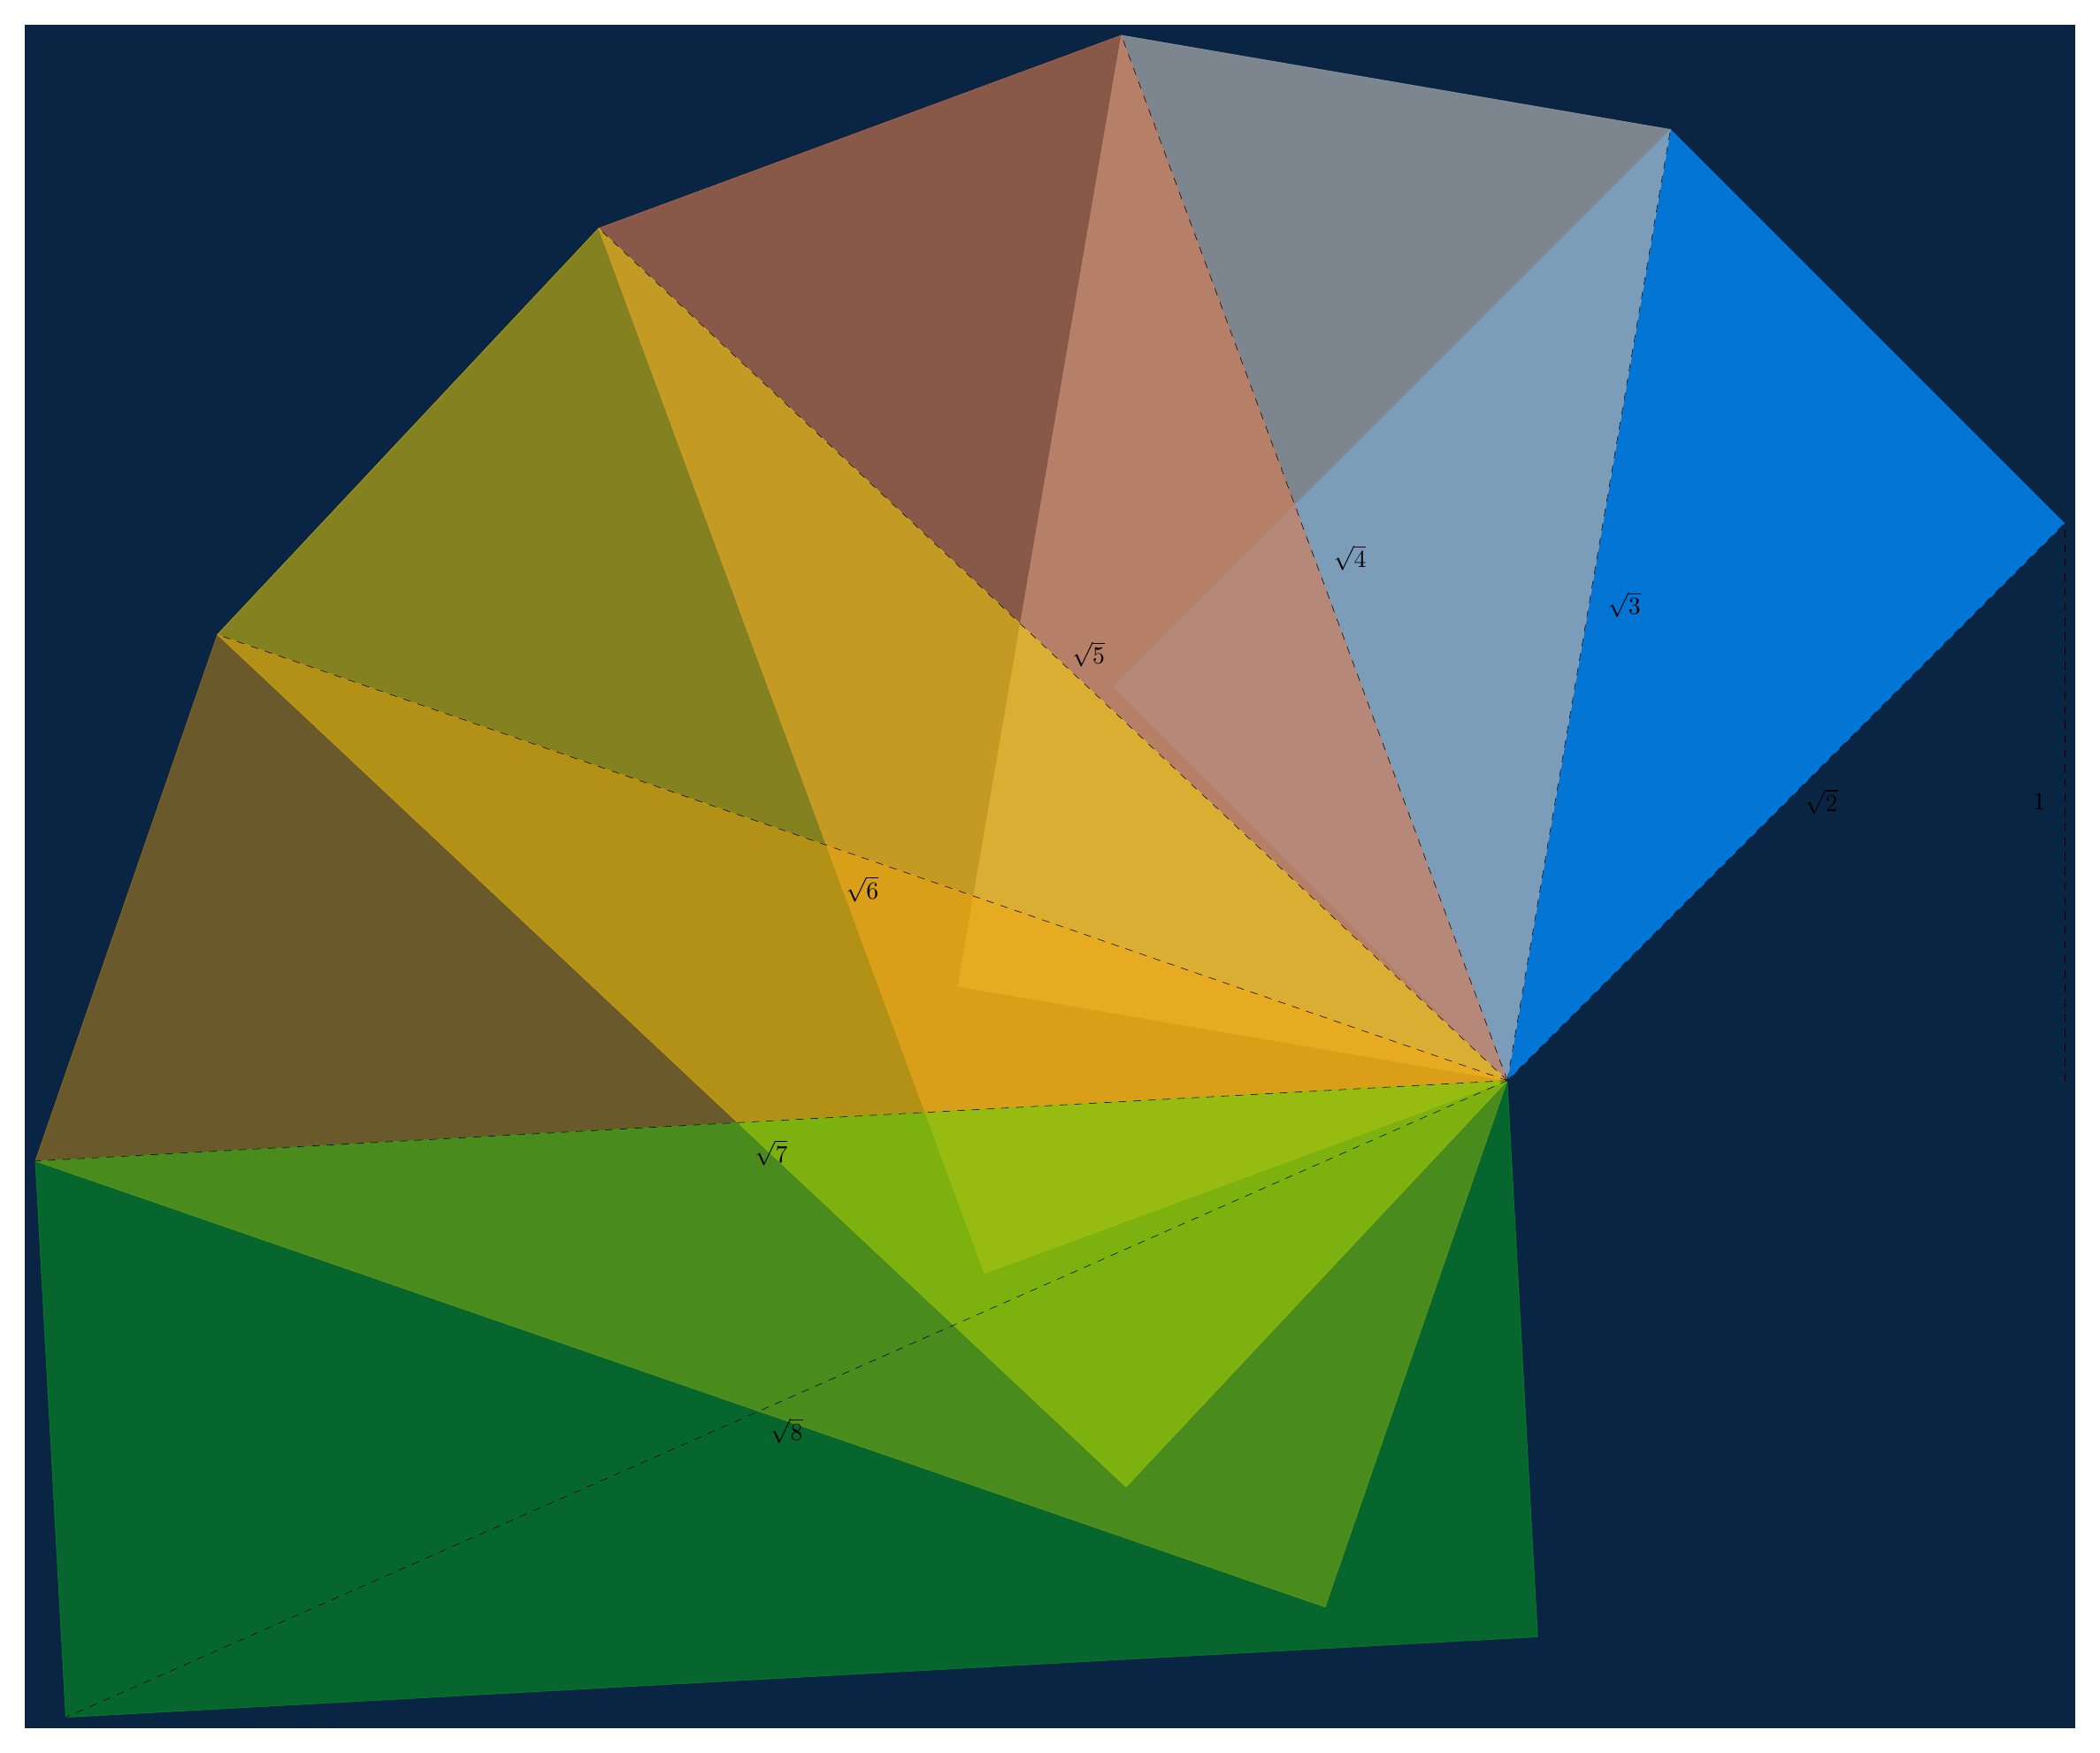
\begin{tikzpicture}[background rectangle/.style={fill=space},show background rectangle]
	%
	\begin{scope}[scale=8]
		\tkzDefPoint(0,0){A}
		\tkzDefPoint(0,1){B}
		\tkzDefSquare(A,B) \tkzGetPoints{C}{D}
		\tkzCalcLength[cm](A,B)\tkzGetLength{lAB}
		\tkzDrawSquare[color=green,fill=green](A,B)
		%
		\tkzDefPointWith[orthogonal normed](D,B) \tkzGetPoint{E}
		\tkzDefPointWith[colinear=at E](D,B) \tkzGetPoint{F}
		\tkzDrawPolygon[color=earth,fill=earth,opacity=0.8](B,D,E,F)
		%
		\tkzDefPointWith[orthogonal normed](D,F) \tkzGetPoint{G}
		\tkzDefPointWith[colinear=at G](D,F) \tkzGetPoint{H}
		\tkzDrawPolygon[color=moon,fill=moon,opacity=0.7](D,F,H,G)
		%
		\tkzDefPointWith[orthogonal normed](D,H) \tkzGetPoint{I}
		\tkzDefPointWith[colinear=at I](D,H) \tkzGetPoint{L}
		\tkzDrawPolygon[color=mars,fill=mars,opacity=0.6](D,H,L,I)
		%
		\tkzDefPointWith[orthogonal normed](D,L) \tkzGetPoint{M}
		\tkzDefPointWith[colinear=at M](D,L) \tkzGetPoint{N}
		\tkzDrawPolygon[color=dida,fill=dida,opacity=0.5](D,L,N,M)
		%
		\tkzDefPointWith[orthogonal normed](D,N) \tkzGetPoint{O}
		\tkzDefPointWith[colinear=at O](D,N) \tkzGetPoint{P}
		\tkzDrawPolygon[color=title,fill=title,opacity=0.4](D,N,P,O)
		%
		\tkzDefPointWith[orthogonal normed](D,P) \tkzGetPoint{Q}
		\tkzDefPointWith[colinear=at Q](D,P) \tkzGetPoint{R}
		\tkzDrawPolygon[color=green,fill=green,opacity=0.3](D,P,R,Q)
		%
		\tkzDrawSegment[dashed](A,B)
		\tkzLabelSegment[black,left=1ex,pos=.5](A,B){$1$}
		%
		\tkzDrawSegment[dashed](D,B)
		\tkzLabelSegment[black,right=1ex,pos=.5](D,B){$\sqrt{2}$}
		%
		\tkzDrawSegment[dashed](D,F)
		\tkzLabelSegment[black,right=1ex,pos=.5](D,F){$\sqrt{3}$}
		%
		\tkzDrawSegment[dashed](D,H)
		\tkzLabelSegment[black,right=1ex,pos=.5](D,H){$\sqrt{4}$}
		%
		\tkzDrawSegment[dashed](D,L)
		\tkzLabelSegment[black,right=1ex,pos=.5](D,L){$\sqrt{5}$}
		%
		\tkzDrawSegment[dashed](D,N)
		\tkzLabelSegment[black,below=1ex,pos=.5](D,N){$\sqrt{6}$}
		%
		\tkzDrawSegment[dashed](D,P)
		\tkzLabelSegment[black,below=1ex,pos=.5](D,P){$\sqrt{7}$}
		%
		\tkzDrawSegment[dashed](D,R)
		\tkzLabelSegment[black,below=1ex,pos=.5](D,R){$\sqrt{8}$}
	\end{scope}
	%
	\end{tikzpicture}
\end{document}